\section{SDN în contextul reţelelor actuale}

Chiar dacă nu este o tehnologie ajunsă la maturitate în toate aspectele unei rețele, paradigma \gls{sdn} este deja folosită în rețele de producție de anumite tipuri. Autorii din \cite{alvizu2017comprehensive} evidenţiază faptul că evoluția \gls{sdn} este susţinută de către trei mari porţiuni ale industriei rețelisticii: furnizorii serviciilor de tip \textit{cloud} (care utilizează mari centre de date), furnizorii de servicii de telecomunicaţii și întreprinderile, așa cum se poate observa și în Figura \ref{fig:sdn_network_deployments}. 

\begin{figure}[h]
	\centering
	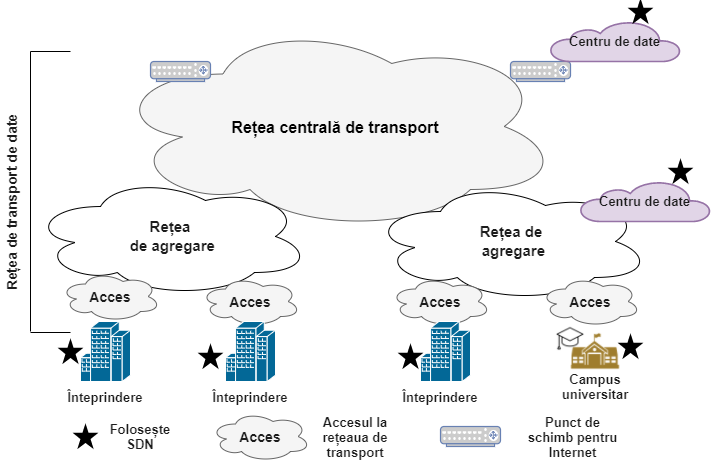
\includegraphics[width=1\textwidth]{sdn_network_deployments}
	\caption{Implementarea SDN în contextul rețelelor actuale~\cite{alvizu2017comprehensive}}
	\label{fig:sdn_network_deployments}
\end{figure}

Astfel, \gls{sdn} este implementat deja cu succes în rețelele unor campusuri universitare (Universitatea Stanford, de exemplu, dat fiind faptul că această paradigmă își are originile acolo), în mari centre de date sau în întreprinderi. În cazul rețelelor de transport, încă se duc activităţi de standardizare care să permită operatorilor rețelelor de telecomunicaţii să implementeze această tehnologie în cel mai scurt timp, beneficiind astfel de avantajele pe care aceasta le oferă (cel mai important, din punctul lor de vedere, fiind reducerea costurilor).

Această secţiune va prezenta în continuare utilizarea \gls{sdn} la momentul actual, în mai multe contexte actuale: în rețelele din marile centre de date, în rețelele de tip hibrid, care combină rețelele tradiționale cu \gls{sdn} sau prin studii de caz, implementări sau experimente efectuate pe teren (în rețele de producție).

\subsection{SDN în centrele de date}

Odată cu apariția tehnologiilor de tip \textit{cloud} și cu ieftinirea puterilor de procesare și de stocare ale calculatoarelor, au apărut centre mari de date, care sunt folosite de către mari furnizori de servicii (precum Google, Facebook, Amazon, etc.). Acestea sunt formate din rețele de servere care conlucrează pentru a oferi diferite tipuri de servicii utilizatorilor. A fost creat astfel un mediu dinamic, atât în cadrul centrelor de date, cât și între acestea. După cum este prezentat și în \cite{onf_openflow_backbone2012}, operații precum prevenirea sau recuperarea în caz de dezastru, sau balansarea încărcării severelor au nevoie de o creștere a traficului între centrele de date, lucru ce duce la o administrare complexa a acelei rețele.

Centrele de date sunt folosite și în cazul oferirii de servicii de virtualizare de servere. Operaţiunile într-un astfel de mediu implică lucrul cu mașini virtuale și, de cele mai multe ori, necesitatea migrării acestora între diferite mașini sau centre de date. Asta înseamnă că diferite aplicații sau servicii trebuie să aibă o vedere proprie asupra rețelei dintre servere, care este doar o vedere la nivel logic, în comparaţie cu rețeaua fizică existentă. Așa cum este prezentat și în \cite{nadeau2013sdn}, crearea de astfel de rețele logice se poate face si fără \gls{sdn}, prin metode folosite și în rețelele tradiționale, cum ar fi cu ajutorul unor \gls{vlan}-uri. Însă, în cazul centrelor de date foarte mari, acestea pot fi insuficiente, astfel că este nevoie și de alte metode.

O metodă pentru crearea de rețele logice care să fie prezentate unor aplicații sau servicii este chiar folosirea tehnologiei \gls{sdn}, făcând abstracţie de rețeaua fizică. În \cite{onf_openflow_backbone2012, onf_sdn_datacenter2013, liu2014sdn, munoz2015integrated} se prezintă diferite metode care pot fi aplicate în astfel de cazuri, sau care chiar au fost demonstrate.

Soluția \gls{sdn} a fost chiar aplicată în rețele de producție. Așa cum se explică în \cite{google_casestudy}, centrele de date ale Google folosesc deja această soluție, cu ajutorul protocolului OpenFlow. Există două laturi ale rețelei de arie largă - \gls{wan} folosită de Google: o parte legată la Internet, care conţine traficul utilizatorilor și o parte internă, care transportă traficul dintre centrele de date. Cele două au caracteristici diferite ale traficului și, implicit, nevoi diferite. În acea rețea internă a fost implementat \gls{sdn}, prin protocolul OpenFlow. Avantajele evidenţiate de Google includ o viziune de ansamblu asupra rețelei, un răspuns mai rapid la erori, timp mai scurt de implementare, actualizări mai rapide ale software-ului rețelei, fără pierdere de trafic sau existența unui mediu de test de mare fidelitate. Chiar dacă în 2012, atunci când a fost implementată această tehnologie în rețea, protocolul OpenFlow era încă la început și nu avea toate facilităţile pe care le oferă astăzi, Google a arătat încă de atunci că tehnologia \gls{sdn} poate fi folosită, aducând foarte multe avantaje, în multe cazuri de utilizare din industria rețelisticii.


\subsection{SDN în rețelele hibride}

\subsection{Studii de caz. Implementări. Experimente în rețele de producție}
